\documentclass[twoside]{book}

% Packages required by doxygen
\usepackage{fixltx2e}
\usepackage{calc}
\usepackage{doxygen}
\usepackage[export]{adjustbox} % also loads graphicx
\usepackage{graphicx}
\usepackage[utf8]{inputenc}
\usepackage{makeidx}
\usepackage{multicol}
\usepackage{multirow}
\PassOptionsToPackage{warn}{textcomp}
\usepackage{textcomp}
\usepackage[nointegrals]{wasysym}
\usepackage[table]{xcolor}

% Font selection
\usepackage[T1]{fontenc}
\usepackage[scaled=.90]{helvet}
\usepackage{courier}
\usepackage{amssymb}
\usepackage{sectsty}
\renewcommand{\familydefault}{\sfdefault}
\allsectionsfont{%
  \fontseries{bc}\selectfont%
  \color{darkgray}%
}
\renewcommand{\DoxyLabelFont}{%
  \fontseries{bc}\selectfont%
  \color{darkgray}%
}
\newcommand{\+}{\discretionary{\mbox{\scriptsize$\hookleftarrow$}}{}{}}

% Page & text layout
\usepackage{geometry}
\geometry{%
  a4paper,%
  top=2.5cm,%
  bottom=2.5cm,%
  left=2.5cm,%
  right=2.5cm%
}
\tolerance=750
\hfuzz=15pt
\hbadness=750
\setlength{\emergencystretch}{15pt}
\setlength{\parindent}{0cm}
\setlength{\parskip}{3ex plus 2ex minus 2ex}
\makeatletter
\renewcommand{\paragraph}{%
  \@startsection{paragraph}{4}{0ex}{-1.0ex}{1.0ex}{%
    \normalfont\normalsize\bfseries\SS@parafont%
  }%
}
\renewcommand{\subparagraph}{%
  \@startsection{subparagraph}{5}{0ex}{-1.0ex}{1.0ex}{%
    \normalfont\normalsize\bfseries\SS@subparafont%
  }%
}
\makeatother

% Headers & footers
\usepackage{fancyhdr}
\pagestyle{fancyplain}
\fancyhead[LE]{\fancyplain{}{\bfseries\thepage}}
\fancyhead[CE]{\fancyplain{}{}}
\fancyhead[RE]{\fancyplain{}{\bfseries\leftmark}}
\fancyhead[LO]{\fancyplain{}{\bfseries\rightmark}}
\fancyhead[CO]{\fancyplain{}{}}
\fancyhead[RO]{\fancyplain{}{\bfseries\thepage}}
\fancyfoot[LE]{\fancyplain{}{}}
\fancyfoot[CE]{\fancyplain{}{}}
\fancyfoot[RE]{\fancyplain{}{\bfseries\scriptsize Generated by Doxygen }}
\fancyfoot[LO]{\fancyplain{}{\bfseries\scriptsize Generated by Doxygen }}
\fancyfoot[CO]{\fancyplain{}{}}
\fancyfoot[RO]{\fancyplain{}{}}
\renewcommand{\footrulewidth}{0.4pt}
\renewcommand{\chaptermark}[1]{%
  \markboth{#1}{}%
}
\renewcommand{\sectionmark}[1]{%
  \markright{\thesection\ #1}%
}

% Indices & bibliography
\usepackage{natbib}
\usepackage[titles]{tocloft}
\setcounter{tocdepth}{3}
\setcounter{secnumdepth}{5}
\makeindex

% Hyperlinks (required, but should be loaded last)
\usepackage{ifpdf}
\ifpdf
  \usepackage[pdftex,pagebackref=true]{hyperref}
\else
  \usepackage[ps2pdf,pagebackref=true]{hyperref}
\fi
\hypersetup{%
  colorlinks=true,%
  linkcolor=blue,%
  citecolor=blue,%
  unicode%
}

% Custom commands
\newcommand{\clearemptydoublepage}{%
  \newpage{\pagestyle{empty}\cleardoublepage}%
}

\usepackage{caption}
\captionsetup{labelsep=space,justification=centering,font={bf},singlelinecheck=off,skip=4pt,position=top}

%===== C O N T E N T S =====

\begin{document}

% Titlepage & ToC
\hypersetup{pageanchor=false,
             bookmarksnumbered=true,
             pdfencoding=unicode
            }
\pagenumbering{roman}
\begin{titlepage}
\vspace*{7cm}
\begin{center}%
{\Large Figures }\\
\vspace*{1cm}
{\large Generated by Doxygen 1.8.11}\\
\end{center}
\end{titlepage}
\clearemptydoublepage
\tableofcontents
\clearemptydoublepage
\pagenumbering{arabic}
\hypersetup{pageanchor=true}

%--- Begin generated contents ---
\chapter{Hierarchical Index}
\section{Class Hierarchy}
This inheritance list is sorted roughly, but not completely, alphabetically\+:\begin{DoxyCompactList}
\item \contentsline{section}{figure}{\pageref{classfigure}}{}
\begin{DoxyCompactList}
\item \contentsline{section}{cercle}{\pageref{classcercle}}{}
\item \contentsline{section}{rectangle}{\pageref{classrectangle}}{}
\item \contentsline{section}{triangle}{\pageref{classtriangle}}{}
\end{DoxyCompactList}
\end{DoxyCompactList}

\chapter{Class Index}
\section{Class List}
Here are the classes, structs, unions and interfaces with brief descriptions\+:\begin{DoxyCompactList}
\item\contentsline{section}{\hyperlink{classcercle}{cercle} \\*Classe cercle, classe fille de figure contenant plusieurs methodes pour calculer la surface et le perimetre du cercle }{\pageref{classcercle}}{}
\item\contentsline{section}{\hyperlink{classfigure}{figure} \\*Classe figure mère contenant plusieurs methodes pour calculer la surface et leperimetre de la figure, classe virtuelle impossible à instancier }{\pageref{classfigure}}{}
\item\contentsline{section}{\hyperlink{classrectangle}{rectangle} \\*Classe rectangle, classe fille de figure contenant plusieurs methodes pour calculer la surface et le perimetre du rectangle }{\pageref{classrectangle}}{}
\item\contentsline{section}{\hyperlink{classtriangle}{triangle} \\*Classe triangle, classe fille de figure contenant plusieurs methodes pour calculer la surface et le perimetre du triangle }{\pageref{classtriangle}}{}
\end{DoxyCompactList}

\chapter{File Index}
\section{File List}
Here is a list of all documented files with brief descriptions\+:\begin{DoxyCompactList}
\item\contentsline{section}{/home/euphoria/\+Documents/cours\+\_\+b2/c\+\_\+c++/b2/figures/src/\hyperlink{cercle_8h}{cercle.\+h} \\*Fichier de la classe cercle }{\pageref{cercle_8h}}{}
\item\contentsline{section}{/home/euphoria/\+Documents/cours\+\_\+b2/c\+\_\+c++/b2/figures/src/\hyperlink{figure_8h}{figure.\+h} \\*Fichier de la classe figure }{\pageref{figure_8h}}{}
\item\contentsline{section}{/home/euphoria/\+Documents/cours\+\_\+b2/c\+\_\+c++/b2/figures/src/\hyperlink{rectangle_8h}{rectangle.\+h} \\*Fichier de la classe rectangle }{\pageref{rectangle_8h}}{}
\item\contentsline{section}{/home/euphoria/\+Documents/cours\+\_\+b2/c\+\_\+c++/b2/figures/src/\hyperlink{triangle_8h}{triangle.\+h} \\*Fichier de la classe cercle }{\pageref{triangle_8h}}{}
\end{DoxyCompactList}

\chapter{Class Documentation}
\hypertarget{classcercle}{}\section{cercle Class Reference}
\label{classcercle}\index{cercle@{cercle}}


classe cercle, classe fille de figure contenant plusieurs methodes pour calculer la surface et le perimetre du cercle  




{\ttfamily \#include $<$cercle.\+h$>$}



Inheritance diagram for cercle\+:\nopagebreak
\begin{figure}[H]
\begin{center}
\leavevmode
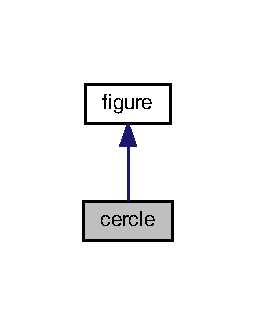
\includegraphics[width=123pt]{classcercle__inherit__graph}
\end{center}
\end{figure}


Collaboration diagram for cercle\+:\nopagebreak
\begin{figure}[H]
\begin{center}
\leavevmode
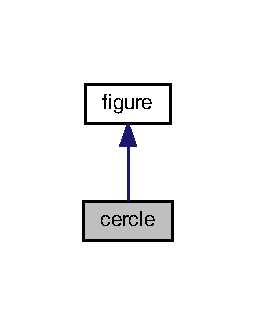
\includegraphics[width=123pt]{classcercle__coll__graph}
\end{center}
\end{figure}
\subsection*{Public Member Functions}
\begin{DoxyCompactItemize}
\item 
float \hyperlink{classcercle_a140f47009fdc3f4ea8c93641538a3778}{surface} (float rayon)\hypertarget{classcercle_a140f47009fdc3f4ea8c93641538a3778}{}\label{classcercle_a140f47009fdc3f4ea8c93641538a3778}

\begin{DoxyCompactList}\small\item\em methode surface, affiche l\textquotesingle{}aire de la figure \textbackslash{} param rayon float \end{DoxyCompactList}\item 
float \hyperlink{classcercle_a55f5bfa84171ffc0c01bd75df6cbf75e}{perimetre} (float rayon)\hypertarget{classcercle_a55f5bfa84171ffc0c01bd75df6cbf75e}{}\label{classcercle_a55f5bfa84171ffc0c01bd75df6cbf75e}

\begin{DoxyCompactList}\small\item\em methode perimetre, affiche le perimetre de la figure \textbackslash{} param rayon float \end{DoxyCompactList}\end{DoxyCompactItemize}


\subsection{Detailed Description}
classe cercle, classe fille de figure contenant plusieurs methodes pour calculer la surface et le perimetre du cercle 

The documentation for this class was generated from the following files\+:\begin{DoxyCompactItemize}
\item 
/home/euphoria/\+Documents/cours\+\_\+b2/c\+\_\+c++/b2/figures/src/\hyperlink{cercle_8h}{cercle.\+h}\item 
/home/euphoria/\+Documents/cours\+\_\+b2/c\+\_\+c++/b2/figures/src/cercle.\+cpp\end{DoxyCompactItemize}

\hypertarget{classfigure}{}\section{figure Class Reference}
\label{classfigure}\index{figure@{figure}}


classe figure mère contenant plusieurs methodes pour calculer la surface et leperimetre de la figure, classe virtuelle impossible à instancier  




{\ttfamily \#include $<$figure.\+h$>$}



Inheritance diagram for figure\+:\nopagebreak
\begin{figure}[H]
\begin{center}
\leavevmode
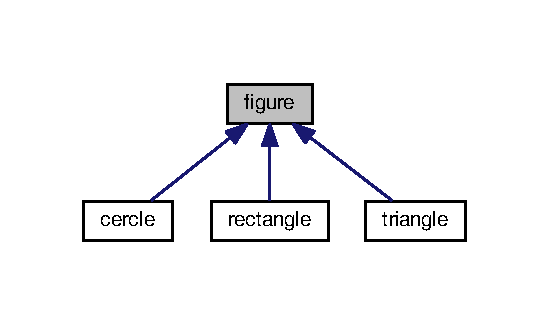
\includegraphics[width=264pt]{classfigure__inherit__graph}
\end{center}
\end{figure}
\subsection*{Public Member Functions}
\begin{DoxyCompactItemize}
\item 
virtual void \hyperlink{classfigure_ad85963e43100c730015701b366755dda}{surface} ()\hypertarget{classfigure_ad85963e43100c730015701b366755dda}{}\label{classfigure_ad85963e43100c730015701b366755dda}

\begin{DoxyCompactList}\small\item\em methode surface, affiche l\textquotesingle{}aire de la figure \end{DoxyCompactList}\item 
virtual void \hyperlink{classfigure_ad6f996a759902c54d77af60047f54e4f}{perimetre} ()\hypertarget{classfigure_ad6f996a759902c54d77af60047f54e4f}{}\label{classfigure_ad6f996a759902c54d77af60047f54e4f}

\begin{DoxyCompactList}\small\item\em methode perimetre, affiche le perimetre de la figure \end{DoxyCompactList}\end{DoxyCompactItemize}


\subsection{Detailed Description}
classe figure mère contenant plusieurs methodes pour calculer la surface et leperimetre de la figure, classe virtuelle impossible à instancier 

The documentation for this class was generated from the following files\+:\begin{DoxyCompactItemize}
\item 
/home/euphoria/\+Documents/cours\+\_\+b2/c\+\_\+c++/b2/figures/src/\hyperlink{figure_8h}{figure.\+h}\item 
/home/euphoria/\+Documents/cours\+\_\+b2/c\+\_\+c++/b2/figures/src/figure.\+cpp\end{DoxyCompactItemize}

\hypertarget{classrectangle}{}\section{rectangle Class Reference}
\label{classrectangle}\index{rectangle@{rectangle}}


classe rectangle, classe fille de figure contenant plusieurs methodes pour calculer la surface et le perimetre du rectangle  




{\ttfamily \#include $<$rectangle.\+h$>$}



Inheritance diagram for rectangle\+:\nopagebreak
\begin{figure}[H]
\begin{center}
\leavevmode
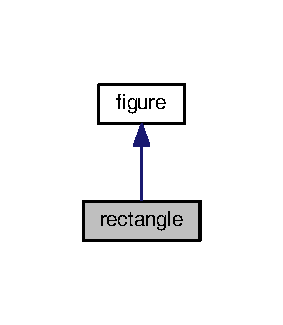
\includegraphics[width=136pt]{classrectangle__inherit__graph}
\end{center}
\end{figure}


Collaboration diagram for rectangle\+:\nopagebreak
\begin{figure}[H]
\begin{center}
\leavevmode
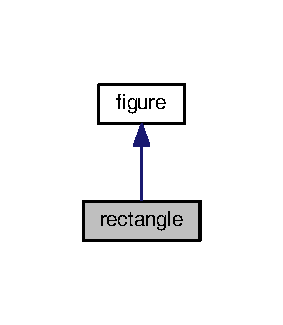
\includegraphics[width=136pt]{classrectangle__coll__graph}
\end{center}
\end{figure}
\subsection*{Public Member Functions}
\begin{DoxyCompactItemize}
\item 
void \hyperlink{classrectangle_a9996c8fd7c082a3cdcea7f6946348794}{surface} (float longueur, float largeur)\hypertarget{classrectangle_a9996c8fd7c082a3cdcea7f6946348794}{}\label{classrectangle_a9996c8fd7c082a3cdcea7f6946348794}

\begin{DoxyCompactList}\small\item\em methode surface, affiche l\textquotesingle{}aire de la figure \textbackslash{} param longueur float \textbackslash{} param largeur float \end{DoxyCompactList}\item 
void \hyperlink{classrectangle_abf7908ec249774c1d68c5285b68271f8}{perimetre} (float longueur, float largeur)\hypertarget{classrectangle_abf7908ec249774c1d68c5285b68271f8}{}\label{classrectangle_abf7908ec249774c1d68c5285b68271f8}

\begin{DoxyCompactList}\small\item\em methode perimetre, affiche le perimetre de la figure \textbackslash{} param longueur float \textbackslash{} param largeur float \end{DoxyCompactList}\end{DoxyCompactItemize}


\subsection{Detailed Description}
classe rectangle, classe fille de figure contenant plusieurs methodes pour calculer la surface et le perimetre du rectangle 

The documentation for this class was generated from the following files\+:\begin{DoxyCompactItemize}
\item 
/home/euphoria/\+Documents/cours\+\_\+b2/c\+\_\+c++/b2/figures/src/\hyperlink{rectangle_8h}{rectangle.\+h}\item 
/home/euphoria/\+Documents/cours\+\_\+b2/c\+\_\+c++/b2/figures/src/rectangle.\+cpp\end{DoxyCompactItemize}

\hypertarget{classtriangle}{}\section{triangle Class Reference}
\label{classtriangle}\index{triangle@{triangle}}


classe triangle, classe fille de figure contenant plusieurs methodes pour calculer la surface et le perimetre du triangle  




{\ttfamily \#include $<$triangle.\+h$>$}



Inheritance diagram for triangle\+:\nopagebreak
\begin{figure}[H]
\begin{center}
\leavevmode
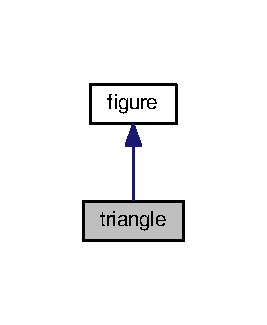
\includegraphics[width=128pt]{classtriangle__inherit__graph}
\end{center}
\end{figure}


Collaboration diagram for triangle\+:\nopagebreak
\begin{figure}[H]
\begin{center}
\leavevmode
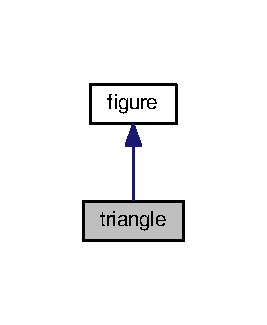
\includegraphics[width=128pt]{classtriangle__coll__graph}
\end{center}
\end{figure}
\subsection*{Public Member Functions}
\begin{DoxyCompactItemize}
\item 
void \hyperlink{classtriangle_ad901747ecf12bd9306efe6b96edb7283}{surface} (float cote1, float cote2, float cote3, float hauteur)\hypertarget{classtriangle_ad901747ecf12bd9306efe6b96edb7283}{}\label{classtriangle_ad901747ecf12bd9306efe6b96edb7283}

\begin{DoxyCompactList}\small\item\em methode surface, affiche l\textquotesingle{}aire de la figure \textbackslash{} param cote1 float \textbackslash{} param cote2 float \textbackslash{} param cote3 float \textbackslash{} param hauteur float \end{DoxyCompactList}\item 
void \hyperlink{classtriangle_a079d90208145fc5cb3f016b42b0ae69d}{perimetre} (float cote1, float cote2, float cote3)\hypertarget{classtriangle_a079d90208145fc5cb3f016b42b0ae69d}{}\label{classtriangle_a079d90208145fc5cb3f016b42b0ae69d}

\begin{DoxyCompactList}\small\item\em methode perimetre, affiche le perimetre de la figure \textbackslash{} param cote1 float \textbackslash{} param cote2 float \textbackslash{} param cote3 float \end{DoxyCompactList}\end{DoxyCompactItemize}


\subsection{Detailed Description}
classe triangle, classe fille de figure contenant plusieurs methodes pour calculer la surface et le perimetre du triangle 

The documentation for this class was generated from the following files\+:\begin{DoxyCompactItemize}
\item 
/home/euphoria/\+Documents/cours\+\_\+b2/c\+\_\+c++/b2/figures/src/\hyperlink{triangle_8h}{triangle.\+h}\item 
/home/euphoria/\+Documents/cours\+\_\+b2/c\+\_\+c++/b2/figures/src/triangle.\+cpp\end{DoxyCompactItemize}

\chapter{File Documentation}
\hypertarget{cercle_8h}{}\section{/home/euphoria/\+Documents/cours\+\_\+b2/c\+\_\+c++/b2/figures/src/cercle.h File Reference}
\label{cercle_8h}\index{/home/euphoria/\+Documents/cours\+\_\+b2/c\+\_\+c++/b2/figures/src/cercle.\+h@{/home/euphoria/\+Documents/cours\+\_\+b2/c\+\_\+c++/b2/figures/src/cercle.\+h}}


fichier de la classe cercle  


{\ttfamily \#include $<$string$>$}\\*
{\ttfamily \#include $<$iostream$>$}\\*
{\ttfamily \#include \char`\"{}figure.\+h\char`\"{}}\\*
Include dependency graph for cercle.\+h\+:\nopagebreak
\begin{figure}[H]
\begin{center}
\leavevmode
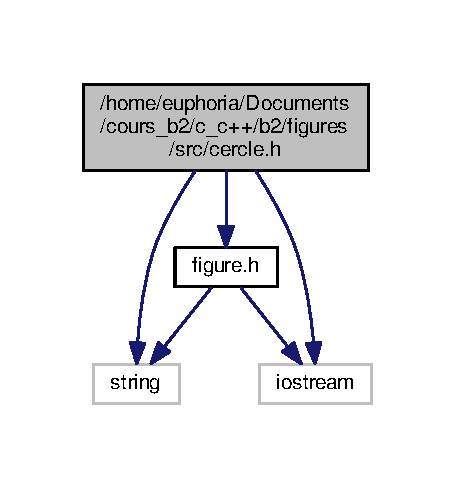
\includegraphics[width=219pt]{cercle_8h__incl}
\end{center}
\end{figure}
\subsection*{Classes}
\begin{DoxyCompactItemize}
\item 
class \hyperlink{classcercle}{cercle}
\begin{DoxyCompactList}\small\item\em classe cercle, classe fille de figure contenant plusieurs methodes pour calculer la surface et le perimetre du cercle \end{DoxyCompactList}\end{DoxyCompactItemize}


\subsection{Detailed Description}
fichier de la classe cercle 

\begin{DoxyAuthor}{Author}
Paul 
\end{DoxyAuthor}
\begin{DoxyVersion}{Version}
1.\+0 
\end{DoxyVersion}

\hypertarget{figure_8h}{}\section{/home/euphoria/\+Documents/cours\+\_\+b2/c\+\_\+c++/b2/figures/src/figure.h File Reference}
\label{figure_8h}\index{/home/euphoria/\+Documents/cours\+\_\+b2/c\+\_\+c++/b2/figures/src/figure.\+h@{/home/euphoria/\+Documents/cours\+\_\+b2/c\+\_\+c++/b2/figures/src/figure.\+h}}


fichier de la classe figure  


{\ttfamily \#include $<$string$>$}\\*
{\ttfamily \#include $<$iostream$>$}\\*
Include dependency graph for figure.\+h\+:\nopagebreak
\begin{figure}[H]
\begin{center}
\leavevmode
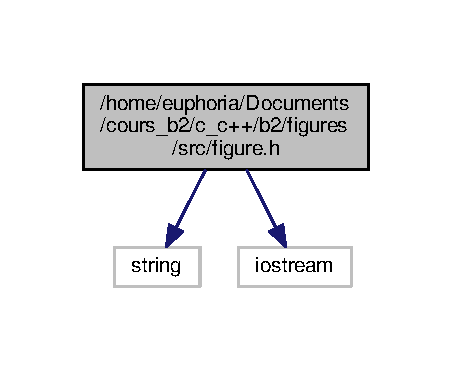
\includegraphics[width=217pt]{figure_8h__incl}
\end{center}
\end{figure}
This graph shows which files directly or indirectly include this file\+:\nopagebreak
\begin{figure}[H]
\begin{center}
\leavevmode
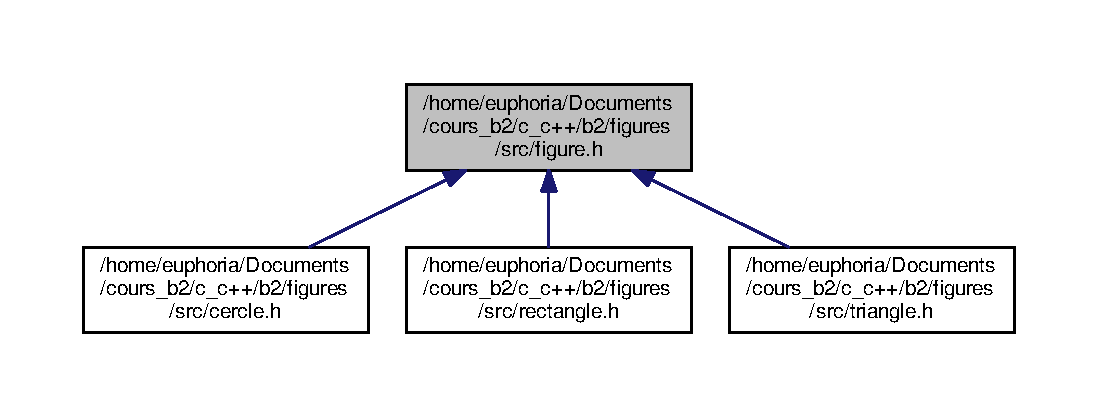
\includegraphics[width=350pt]{figure_8h__dep__incl}
\end{center}
\end{figure}
\subsection*{Classes}
\begin{DoxyCompactItemize}
\item 
class \hyperlink{classfigure}{figure}
\begin{DoxyCompactList}\small\item\em classe figure mère contenant plusieurs methodes pour calculer la surface et leperimetre de la figure, classe virtuelle impossible à instancier \end{DoxyCompactList}\end{DoxyCompactItemize}


\subsection{Detailed Description}
fichier de la classe figure 

\begin{DoxyAuthor}{Author}
Paul 
\end{DoxyAuthor}
\begin{DoxyVersion}{Version}
1.\+0 
\end{DoxyVersion}

\hypertarget{rectangle_8h}{}\section{/home/euphoria/\+Documents/cours\+\_\+b2/c\+\_\+c++/b2/figures/src/rectangle.h File Reference}
\label{rectangle_8h}\index{/home/euphoria/\+Documents/cours\+\_\+b2/c\+\_\+c++/b2/figures/src/rectangle.\+h@{/home/euphoria/\+Documents/cours\+\_\+b2/c\+\_\+c++/b2/figures/src/rectangle.\+h}}


fichier de la classe rectangle  


{\ttfamily \#include $<$string$>$}\\*
{\ttfamily \#include $<$iostream$>$}\\*
{\ttfamily \#include \char`\"{}figure.\+h\char`\"{}}\\*
Include dependency graph for rectangle.\+h\+:\nopagebreak
\begin{figure}[H]
\begin{center}
\leavevmode
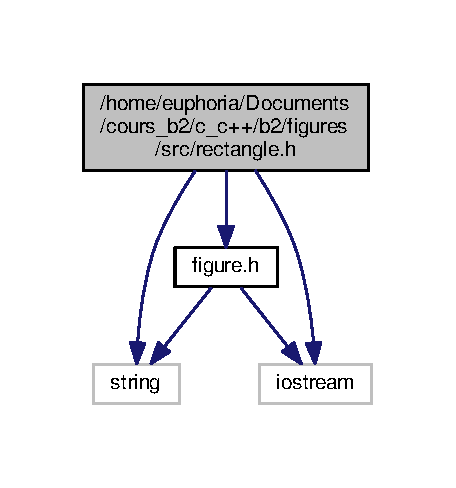
\includegraphics[width=219pt]{rectangle_8h__incl}
\end{center}
\end{figure}
\subsection*{Classes}
\begin{DoxyCompactItemize}
\item 
class \hyperlink{classrectangle}{rectangle}
\begin{DoxyCompactList}\small\item\em classe rectangle, classe fille de figure contenant plusieurs methodes pour calculer la surface et le perimetre du rectangle \end{DoxyCompactList}\end{DoxyCompactItemize}


\subsection{Detailed Description}
fichier de la classe rectangle 

\begin{DoxyAuthor}{Author}
Paul 
\end{DoxyAuthor}
\begin{DoxyVersion}{Version}
1.\+0 
\end{DoxyVersion}

\hypertarget{triangle_8h}{}\section{/home/euphoria/\+Documents/cours\+\_\+b2/c\+\_\+c++/b2/figures/src/triangle.h File Reference}
\label{triangle_8h}\index{/home/euphoria/\+Documents/cours\+\_\+b2/c\+\_\+c++/b2/figures/src/triangle.\+h@{/home/euphoria/\+Documents/cours\+\_\+b2/c\+\_\+c++/b2/figures/src/triangle.\+h}}


fichier de la classe cercle  


{\ttfamily \#include $<$string$>$}\\*
{\ttfamily \#include $<$iostream$>$}\\*
{\ttfamily \#include \char`\"{}figure.\+h\char`\"{}}\\*
Include dependency graph for triangle.\+h\+:\nopagebreak
\begin{figure}[H]
\begin{center}
\leavevmode
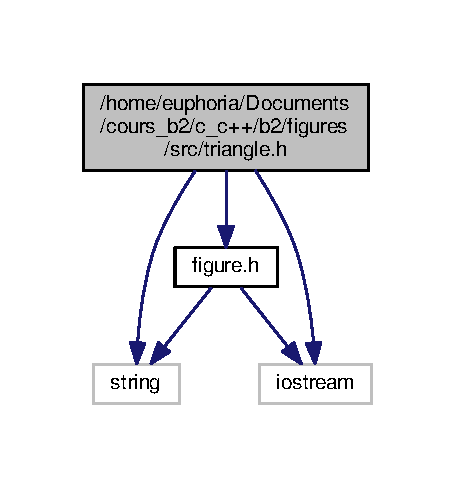
\includegraphics[width=219pt]{triangle_8h__incl}
\end{center}
\end{figure}
\subsection*{Classes}
\begin{DoxyCompactItemize}
\item 
class \hyperlink{classtriangle}{triangle}
\begin{DoxyCompactList}\small\item\em classe triangle, classe fille de figure contenant plusieurs methodes pour calculer la surface et le perimetre du triangle \end{DoxyCompactList}\end{DoxyCompactItemize}


\subsection{Detailed Description}
fichier de la classe cercle 

\begin{DoxyAuthor}{Author}
Paul 
\end{DoxyAuthor}
\begin{DoxyVersion}{Version}
1.\+0 
\end{DoxyVersion}

%--- End generated contents ---

% Index
\backmatter
\newpage
\phantomsection
\clearemptydoublepage
\addcontentsline{toc}{chapter}{Index}
\printindex

\end{document}
